\section{Method}
\subsection{Preparations}

The preparations consisted mainly of choosing which sensor to choose for the detection of the ball and how to mount it to the balance beam. Using the built in plotter of the Arduino IDE we compared an ultrasonic sensor and IR-sensors noise and accuracy. The result was that the IR-sensor was more consistent and linear than the ultrasonic sensor, thus easier to regulate.

After concluding towards the IR-sensor, the group decided to create several sensor mounts. The sensor mounts were printed with a vertical sensor orientation with different sensor heights. Therefore the group could do further test to see what height the IR-sensor was the most effective and consistent at a stable position. 

In a vertical position, the IR-sensor was not perfectly lined up with the center of the ball, due to the the size of the sensor. This lead to misreading across the span of the beam. The group concluded to again change the wall mount. By mounting the sensor horizontally, the sensor aligned with the middle of the ball and the scaling issue was resolved. To calibrate the sensor, the group used a ruler to validate the distance readings against actual distance and were happy with the result provided by the general equation \ref{eq:sharp-linear}.

The group also concluded to flip the servomotor. This placed the connection point between the pole and balance beam closer towards the rotation point, resulting in a greater possible angle span on the balance beam. After connecting a 5-volt voltage regulator to the servo motor and a capacitor to the IR sensor, the preparations was finished and the group could continue with the regulation of the system. 
\subsection{Circuit}
The main components of the electronic circuit were an Arduino UNO, breadboard, servo motor and a sharp distance sensor. In order to run the servo motor on the correct voltage we used a L7805, 5 volt voltage regulator. The capacitors are included as described in the datasheets of the LM7805 \cite{LM78XX-datasheet} and the Sharp IR-sensor \cite{Sharp-datasheet} to reduce electrical noise.

\begin{figure}[h]
    \centering
    \includegraphics[width = 1\textwidth]{Images/Circuit-snip.png}
    \caption{Circuit design}
    \label{fig:Circuit design}
\end{figure}

\subsection{PID controller}


The group started by looking at different examples of Arduino libraries for the PID controller. After reading through and testing multiple different libraries, the group decided to manually code the controller. This also made it possible to add a threshold to the I-term.

\begin{equation}
    h(s) = \frac{r(s)}{\theta(s)}\ = \frac{mg\frac{d}{L}}{(\frac{J}{R^2}+m)s^2}
\end{equation}

Even though the IR-sensor had significantly less noise than the ultrasonic sensor, it was still enough to cause reading errors. Therefore the group decided to implement digital filters to the code. The implemented filters was a Kalman filter and a Median filter, both used to minimize noise in the sensor readings. 

However, as discussed in several classes, it is hard to make a perfect mathematical model of a practical problem. In the end the group concluded that trial and error for the parameter values was the way to go. The parameters that needed to be adjusted were Kp, Ki, Kd, sample rate, Kalman filter, threshold and mapping of PID. After several hours of testing, discussion and plotting in MATLAB, the group used the following values for the mentioned parameters.\\

\begin{tabular}{r l}
 
 PID: \\
    $K_p$ & 6\\
    $K_i$ & 0.15\\
    $K_d$ & 5000\\
    
    \\
    \hline
    \\

Kalman filter: \\
    Measurement uncertainty, $KF_{mea}$ & 1.2 \\
    Estimation uncertainty, $KF_{est}$ & 2 \\
    Process Variance, $KF_{var}$ & 0.3\\ \\
    \hline
    \\
Median filter:\\
    Window size & 5\\
    \\
    \hline
    \\
General: \\
Threshold for the ball to settle(cm) & 0 $<$ threshold $<$ 1\\
Mapping of PID & (240, -240)\\
Constrain of servo position & (15, 95)\\
Sample rate & 25\\
\end{tabular}

The group discovered that removing the integral constant from the PID massively reduced the settling time but proportionally increased the steady state error. Creating a threshold for the integral part of the PID to operate was an attempt to reduce the impact of the constant on the rest of the system, without removing it completely. 

As the ball entered the threshold some problems occurred. The IR-sensor still had minor noises even though the group implemented filters. Due to inconsistent sensor values, the settling time inside the threshold was slow. The group tried to solve this problem by adding a timer to the system. As the ball entered the set threshold, the PID was given a one second operating time before locking the output to the servo position. This resulted in a fast settling time but a small inconsistent steady state inside that threshold.

The group aimed for the "excellent" requirements given in the task. In order to mitigate every factor we had to make a trade off. The following goals were given:
\begin{center}
\begin{tabular}{ |c|c|c|c|}
 \hline
 Requirements & Excellent & Good & Fair \\
 \hline
 Stabilization time & $<$ 3 secs & $<$ 5 secs & $>$ 5 secs\\ 
 \hline
 Overshoot & $<$ 3 cm & $<$ 5 cm & $>$ 5 cm \\  
 \hline
 Oscillations in SS & None & $<$ +/- 5mm & $>$ +/- 5mm \\
 \hline
 Steady state error & $<$ 1 cm & $<$ 2 cm & $>$ 2 cm \\
 \hline
 Other & - & - & - \\
 \hline
\end{tabular}
\end{center}

\subsection{MATLAB analysis}

Appendix \ref{apx:matlab} shows the MATLAB code to analyse the system. The results were as expected and shows that we have chosen a configuration with a quick settling time and without overshoot.

The closed loop transfer function is calculated using Matlab.
\begin{equation}
    TF = \frac{19.87s^2+0.02384s+0.000596}{1.803s^3+19.87s^2+0.2384s+0.000596}
\end{equation}

\begin{figure}[H]
    \caption{Plot of the transfer function of the system}
    \centering
    \begin{subfigure}[t]{0.48\textwidth}
        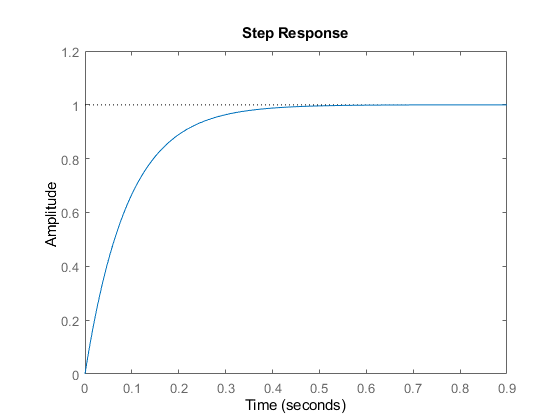
\includegraphics[width = \textwidth]{Images/Matlab_StepResponse.png}
        \caption{Step response, with PID-controller}
        \label{fig:Step-PID-control}
    \end{subfigure}
    \begin{subfigure}[t]{0.48\textwidth}
        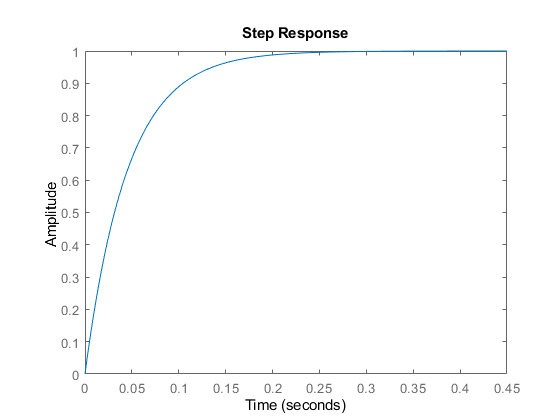
\includegraphics[width = \textwidth]{Images/Matlab_StepResponse_D-controller.png}
        \caption{Step response, example with only D-controller}
        \label{fig:Step-D-control}
    \end{subfigure}  
\end{figure}


The step response, \ref{fig:Step-PID-control}, reveals a quick settling time and no overshoot. This is when using the P, I and D parameters that are used on the physical model. 

The poles of the closed loop system are 
$$ p_1 = -11.0185 $$ 
$$ p_2 = -0.0006 + 0.0054i $$ 
$$ p_3 = -0.0006 - 0.0054i $$
where $p_2$ and $p_3$ are dominant ones. All poles being negative means that the closed loop system is stable. Looking at the step-response, this seams to be right 

In figure \ref{fig:Step-D-control}, the mathematical model is ran with only the D-term active, with a value of 10000. The mathematical model shows a greater settling time. However, when testing those controller-parameters on the physical model, the response was worse. A great example that the mathematical model may not always be a true representation.
